\begin{filecontents}{ph4.dat}
X Sample  	Hanna  DFRobot	
1 1         	4.4	4.3
2 2         	4.4	4.4
3 3         	4.4	4.4
4 4         	4.4	4.4
5 5         	4.4	4.4
\end{filecontents}

\begin{filecontents}{ph7.dat}
X Sample  	Hanna  DFRobot	
1 1         	7.2	7.3
2 2         	7.2	7.3
3 3         	7.2	7.3
4 4         	7.3	7.3
5 5         	7.2	7.3
\end{filecontents}

\begin{filecontents}{ec1288.dat}
X Sample  	DFRobot   Mean
1 1         	13.3   13.06
2 2         	13.0
3 3         	13.0
4 4         	12.9
5 5         	13.1   13.06
\end{filecontents}

\begin{filecontents}{ec1433.dat}
X Sample  	DFRobot   Mean
1 1         	1.6   1.56
2 2         	1.5
3 3         	1.6
4 4         	1.6
5 5         	1.5   1.56
\end{filecontents}

\begin{filecontents}{temp.dat}
X Sample  	Hanna  DFRobot	
1 1         	30.3 31.12
2 2         	30.4 31.44
3 3         	30.3 32.06
4 4         	30.5 32.13
5 5         	30.7 32.38
\end{filecontents}
\subsection{Sensors}

The sensor package on the drone is equipped with a turbidity, conductivity, and acidity meter. A minimum accuracy and range requirement for these sensors will be established based on an use case provided by PERNAM \gls{JSC}. Accuracy of these parameters will be measured both in the laboratory and in practice. All sensors are calibrated accordingly beforehand. A full morphological overview of the sensors can be found in the preliminary research report (Appendix A)

\subsubsection{Use case} \label{sensors:usecase}

PERNAM \gls{JSC} wishes to use an \gls{UAV} that has the capability to measure the turbidity, conductivity, and acidity around their water filtration plants in hopes to detect anomalies in the water input early on. For the system to be useful, they have listed some accuracy requirements as follows:

\begin{description}
   \item[Acidity] 2\% of full scale range so +/- 0.3pH
   \item[Conductivity] 5\% of full scale range so +/- 5ms/cm
   \item[Turbidity] 5\% of full scale range so +/- 150NTU
\end{description}

As seen in the tests below, the chosen sensors are accurate enough for PERNAM's use case.

\newpage
\subsubsection{Acidity} \label{sensors:acidity}

As mentioned in the Design Report, the DFRobot SEN0169 V2 Pro \cite{SEN0169V2} was chosen for measuring the acidity. The manufacturer claims the sensor has a resolution of 0.1pH across the whole range from 0 to 14pH.

\begin{figure}[h]
  \centering
  \begin{minipage}[b]{0.4\textwidth}
    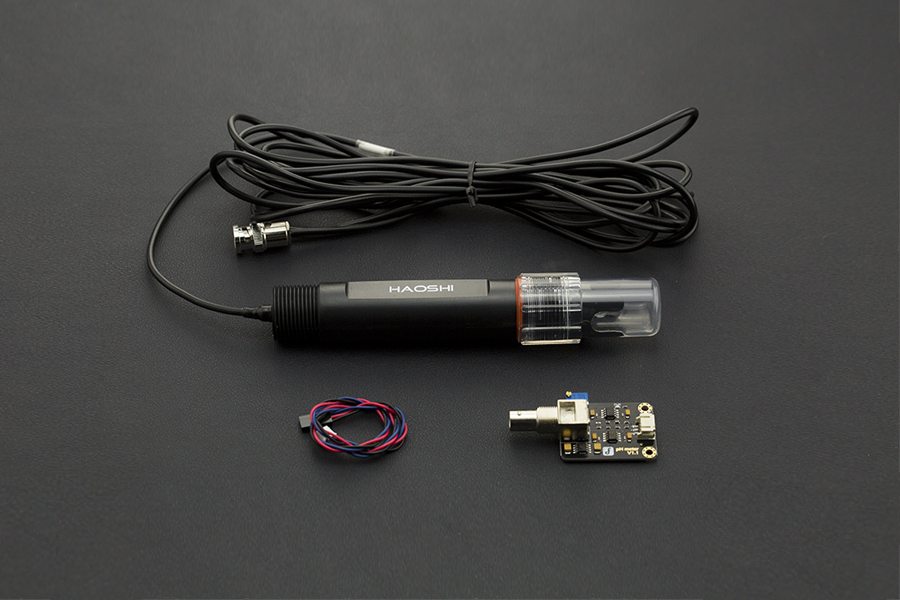
\includegraphics[width=\textwidth]{080_testing/sensors/12_gravityv2pro.jpg}
    \caption{SEN0169 V2 Pro \cite{SEN0169V2}}
  \end{minipage}
  \hfill
  \begin{minipage}[b]{0.3\textwidth}
    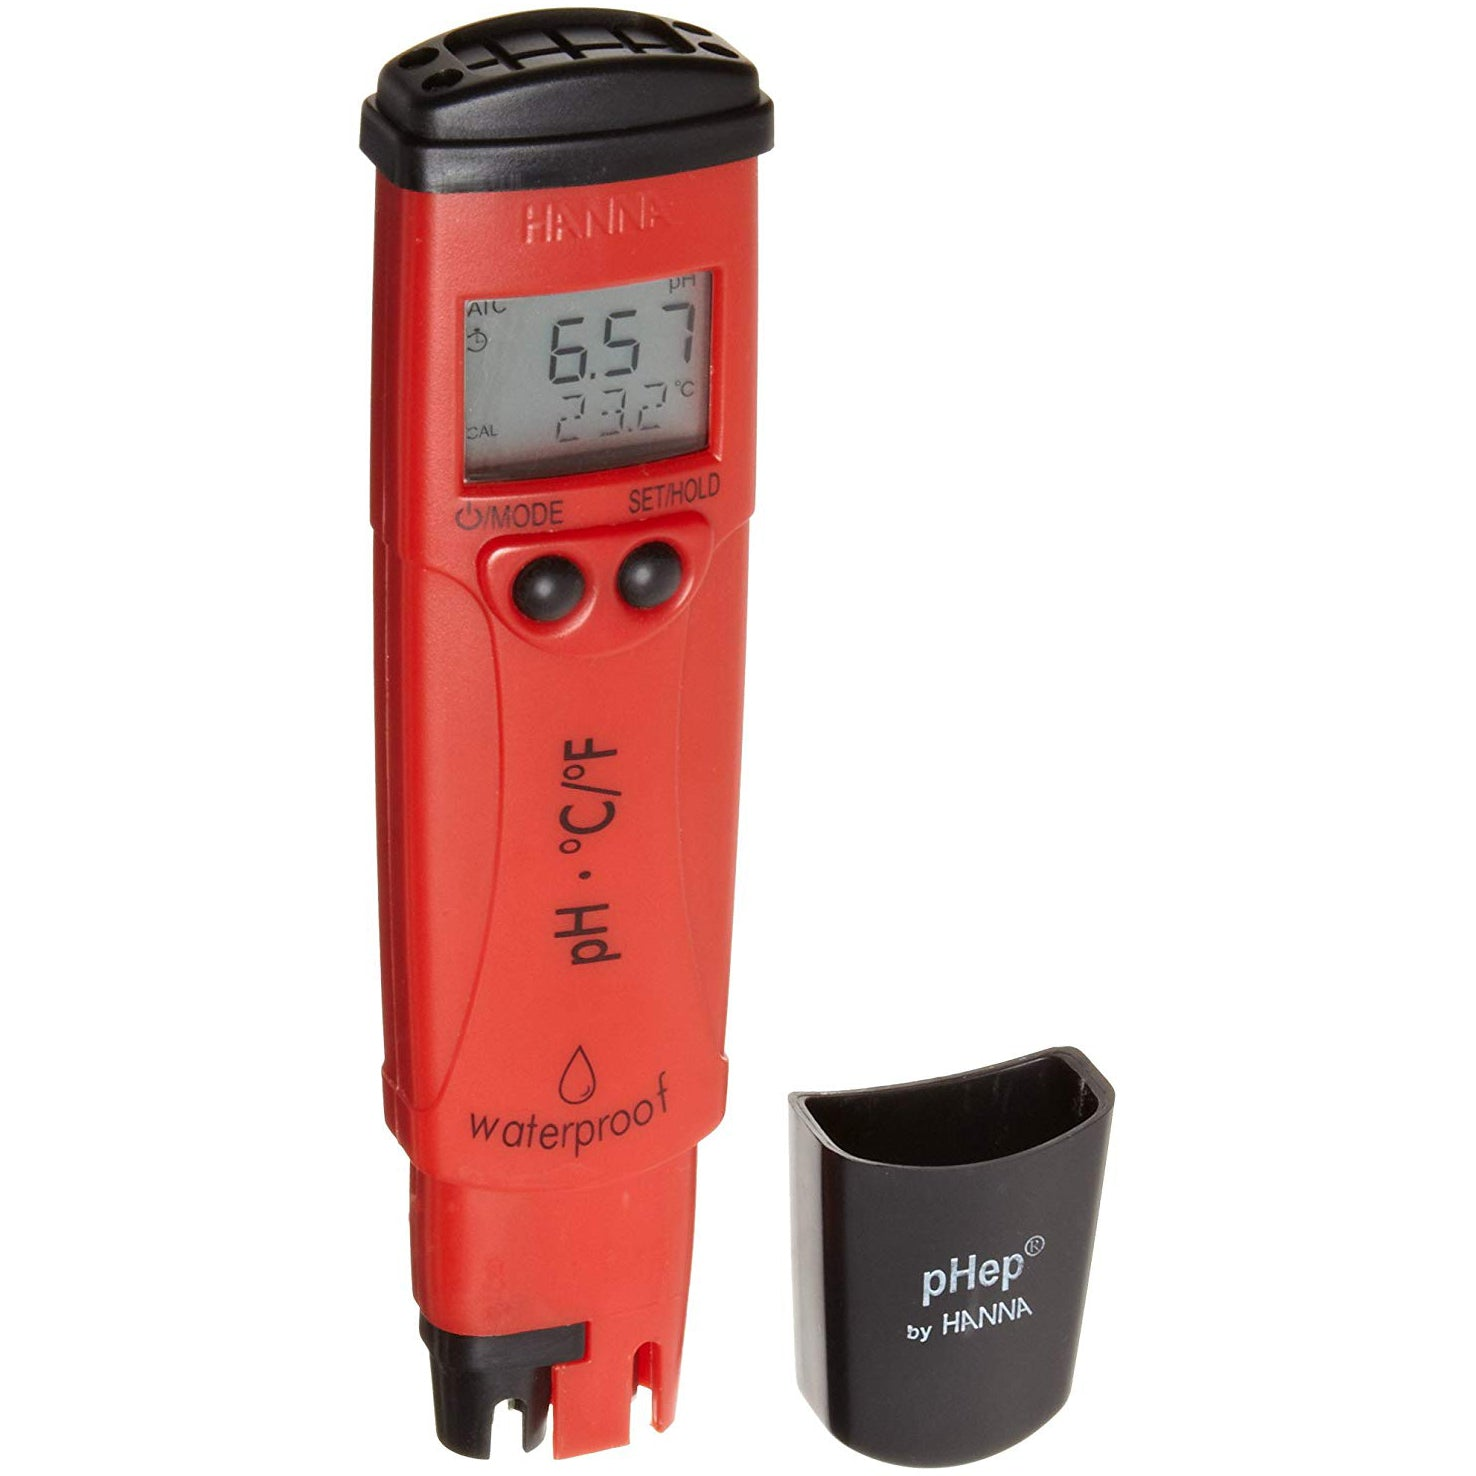
\includegraphics[width=\textwidth]{080_testing/sensors/11_hanna.jpg}
    \caption{Hanna pHep \cite{hanna}}
  \end{minipage}
\end{figure}

The chosen sensor was compared against the Hanna pHep, that also has a resolution of 0.1pH. \cite{hanna} Two solutions with different pH were tested on both sensors. Before each sample was taken, both sensors were cleaned with distilled water. A sample is taken a minute after submersion, as the response time of both acidity sensors are within 1 minute.

\newpage
\paragraph{First solution}
The first solution is marked in pink.

\begin{figure}[h]
  \centering
  \begin{minipage}[b]{0.2\textwidth}
    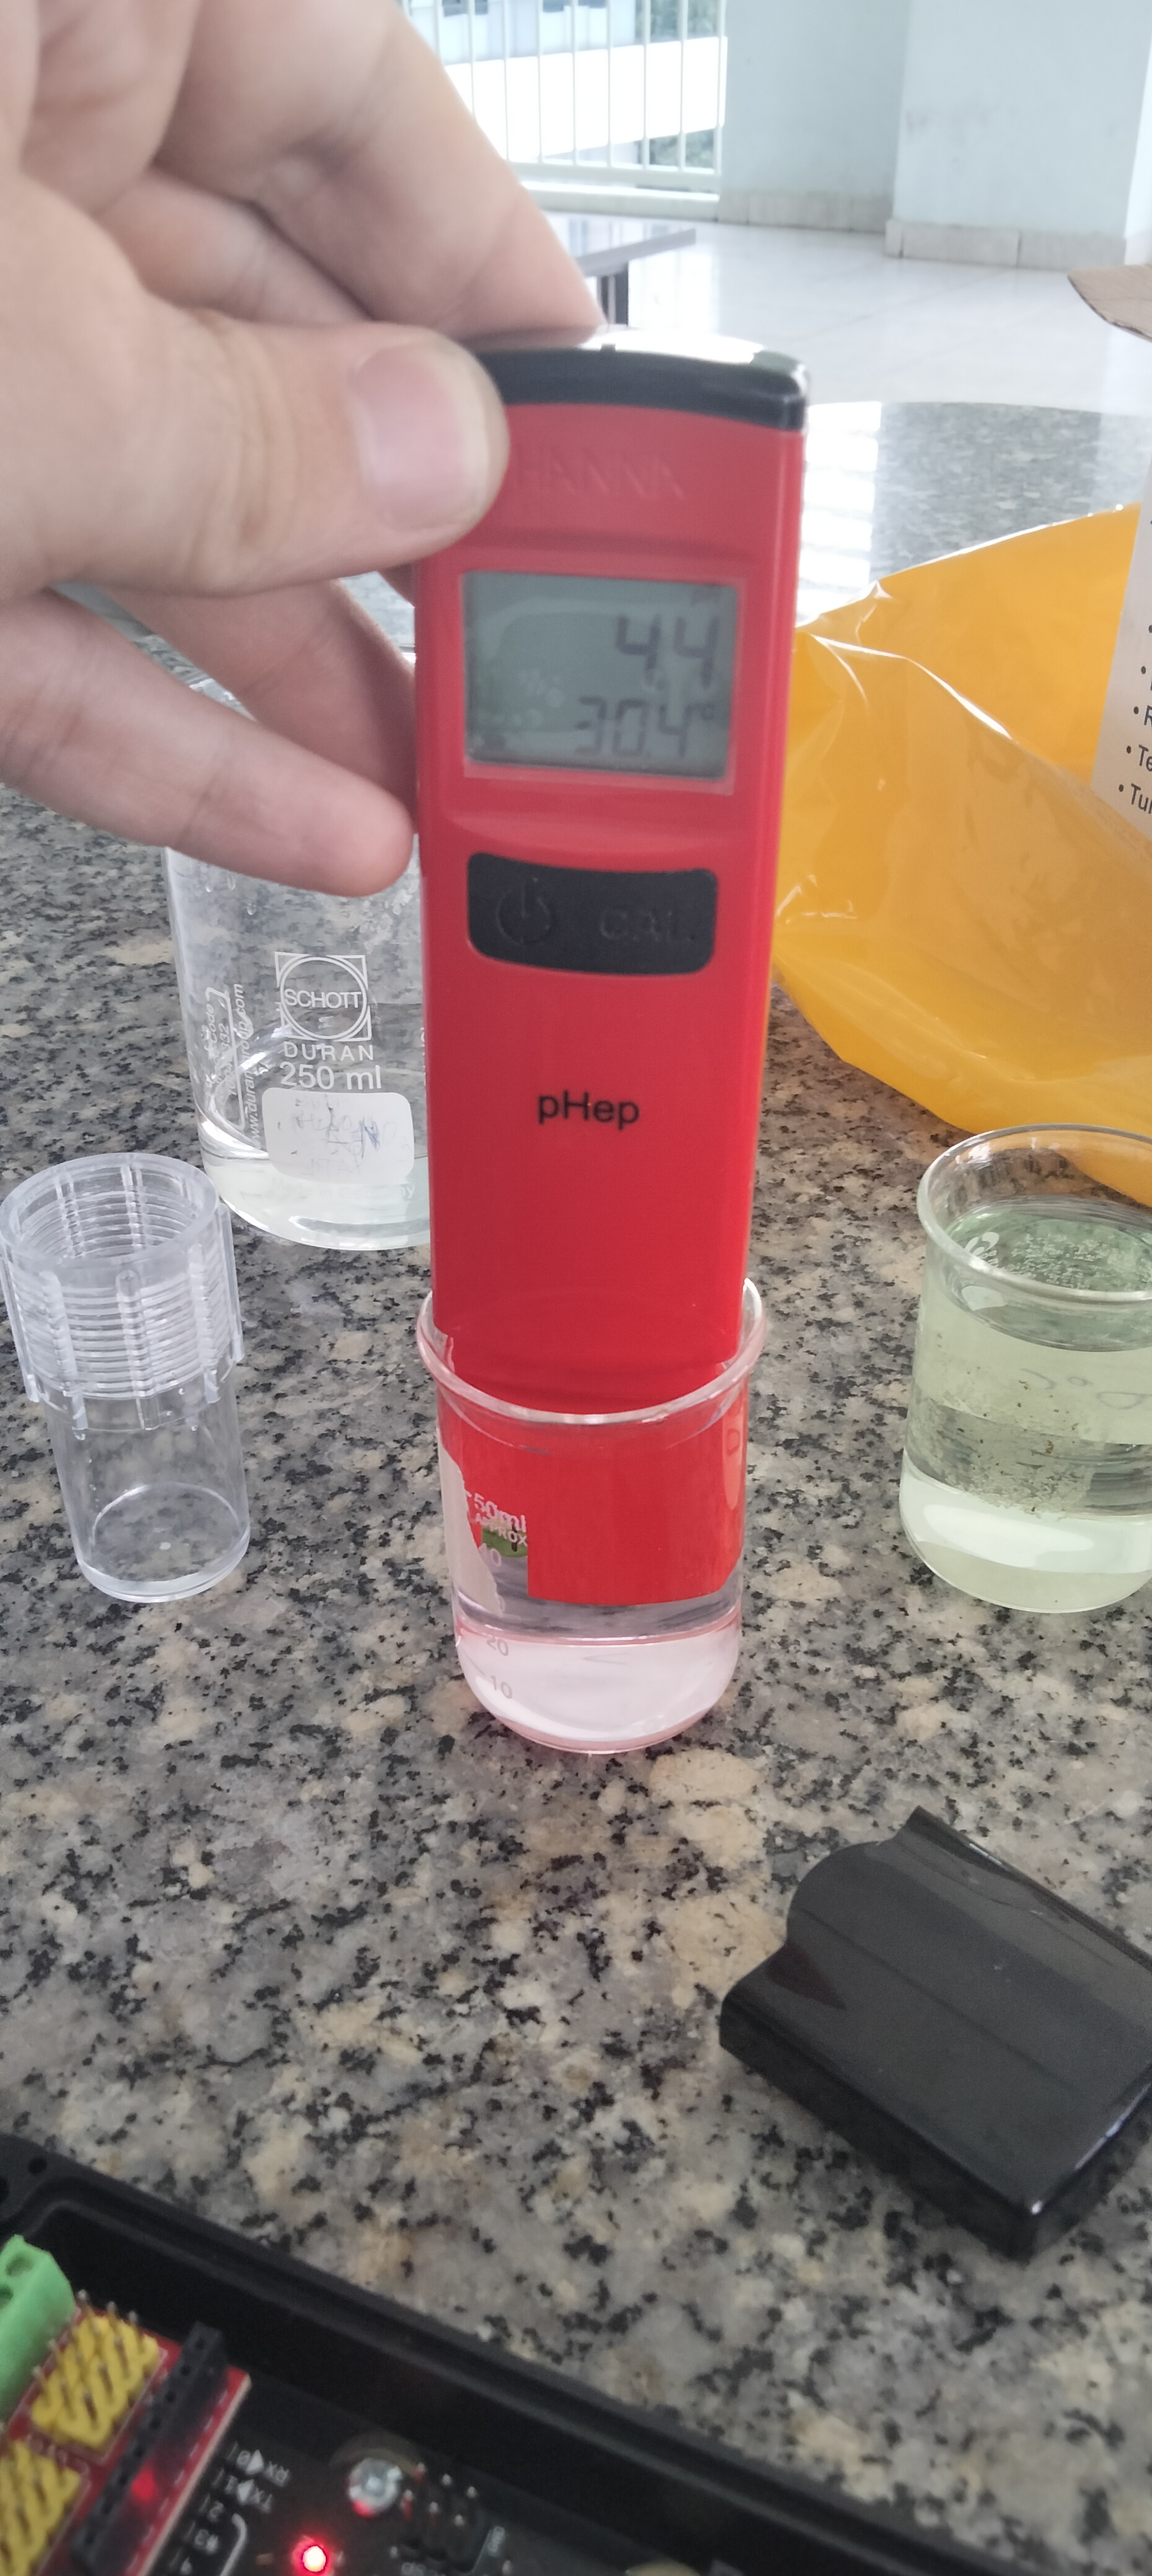
\includegraphics[width=\textwidth]{080_testing/sensors/14_ph4_hanna.jpg}
    \caption{Hanna sensor measuring 4.4}
  \end{minipage}
  \hfill
  \begin{minipage}[b]{0.7\textwidth}
    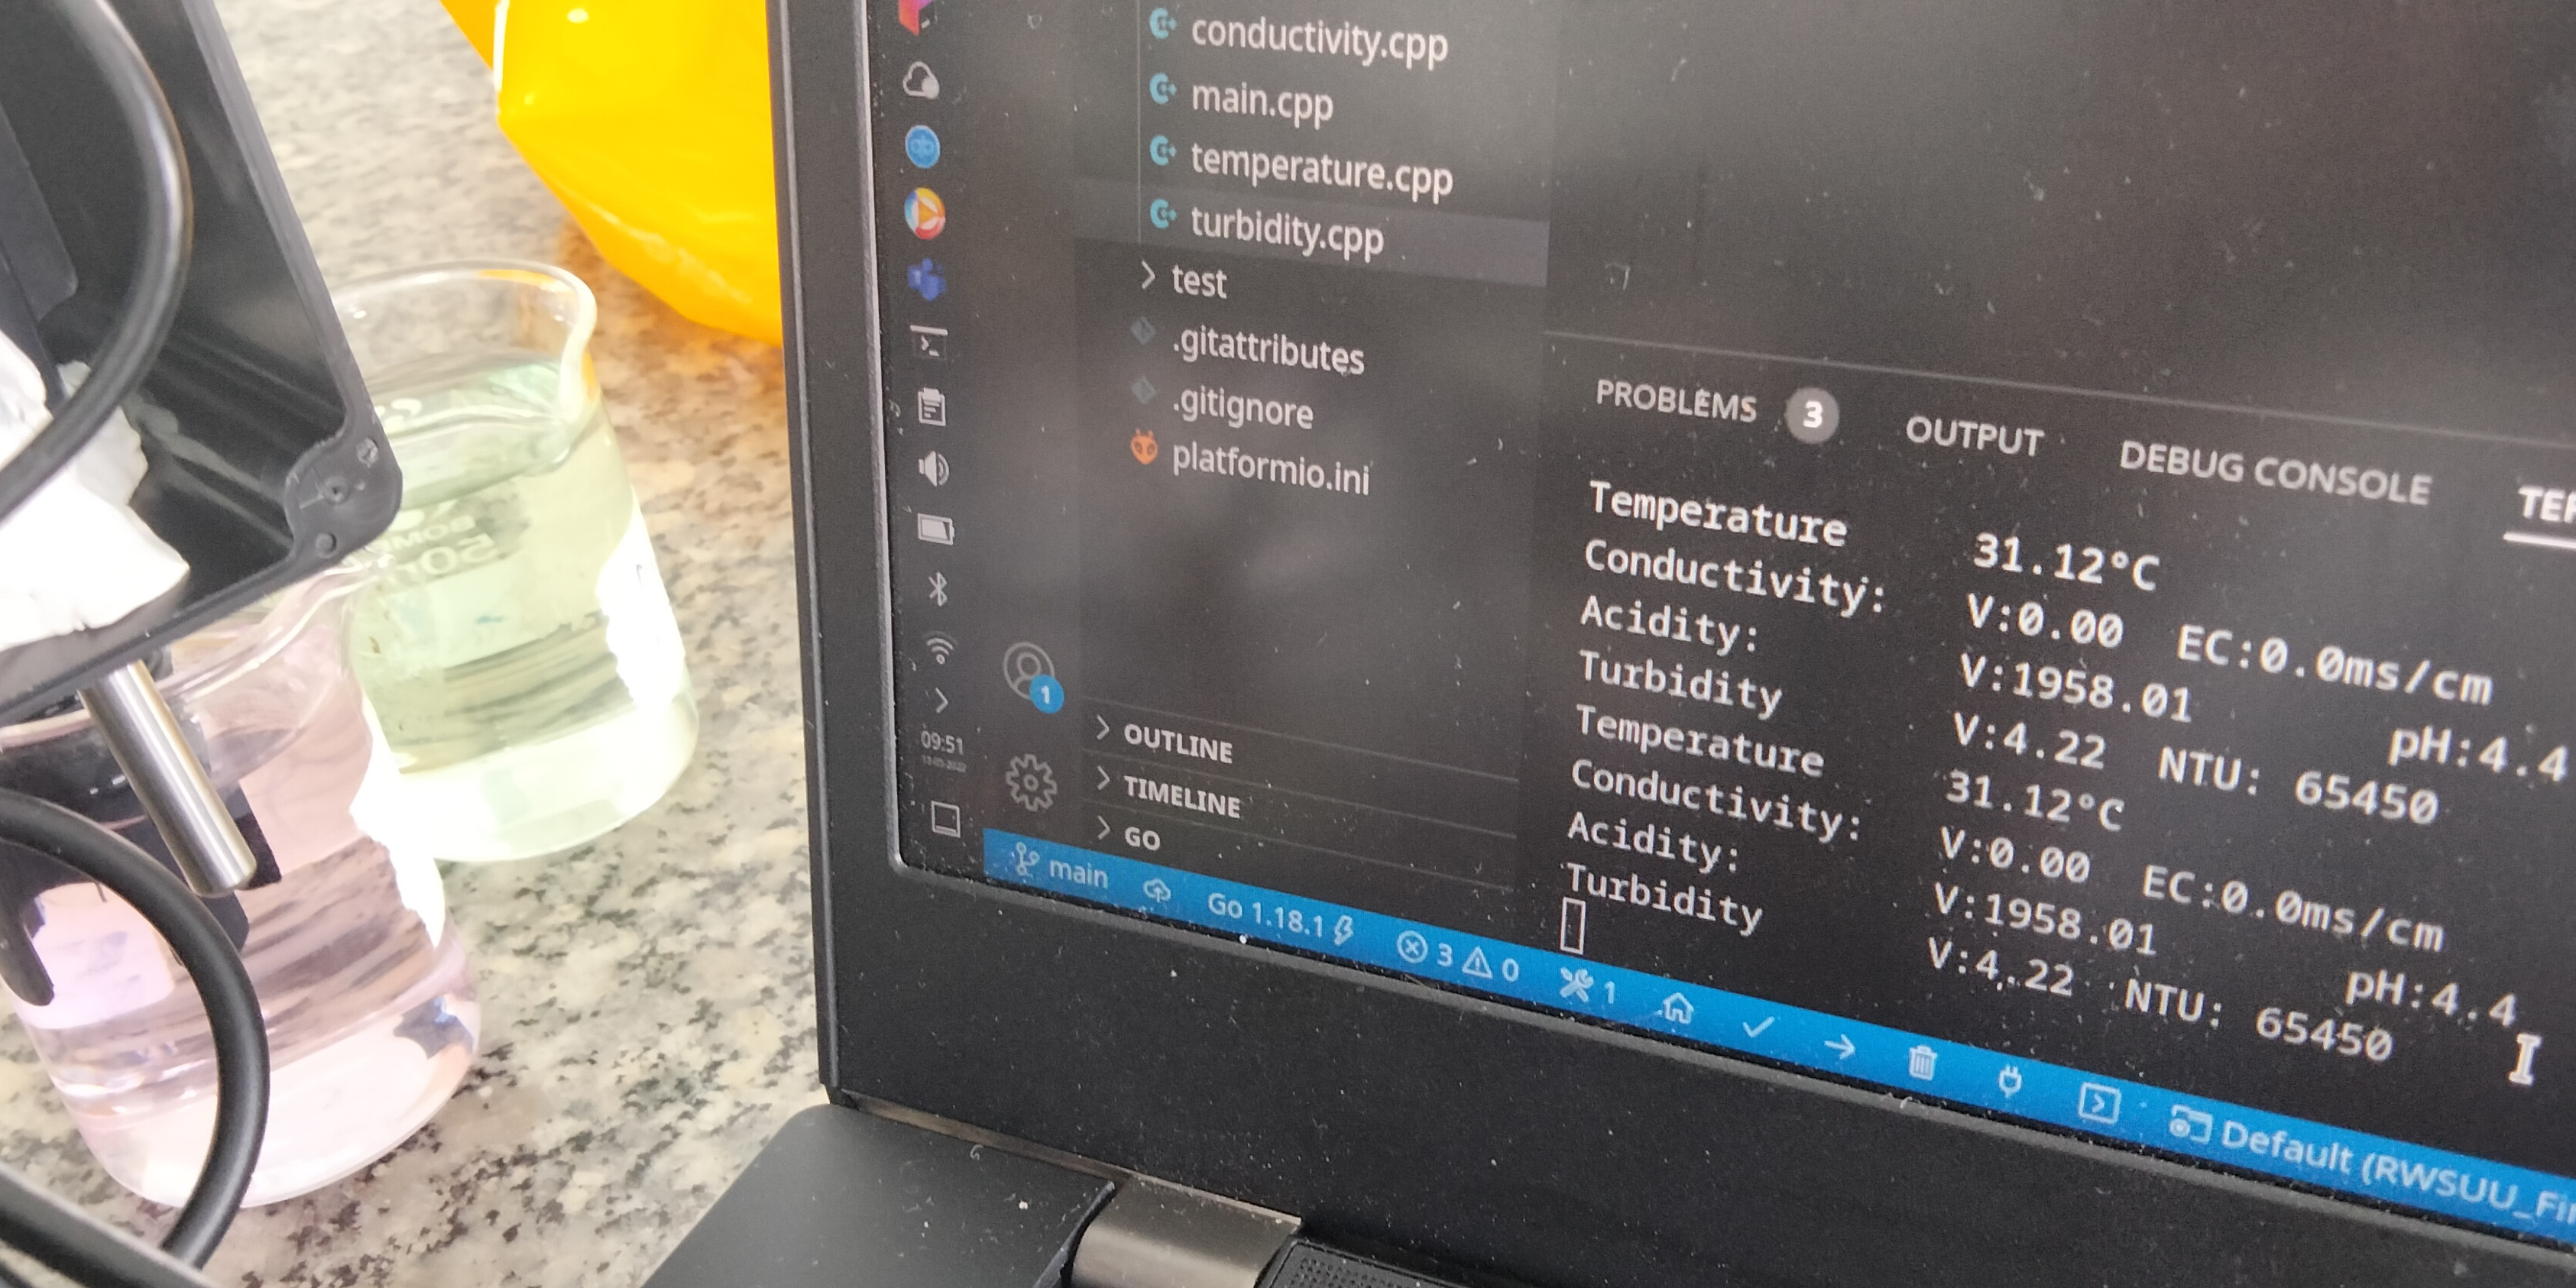
\includegraphics[width=\textwidth]{080_testing/sensors/13_ph4_dfrobot.jpg}
    \caption{DFRobot sensor measuring 4.4}
  \end{minipage}
\end{figure}

\begin{figure}[h!]
\caption{Comparison between Hanna and DFRobot on pH 4.4}
\begin{tikzpicture}
\begin{axis}[
axis lines=middle,
ymin=0,
x label style={at={(current axis.right of origin)},anchor=north, below=10mm},
legend style={at={(0.7,0.7)},anchor=east},
ymin=4, ymax=5,
    xlabel=Samples,
  ylabel=pH,
   enlargelimits = true,
  xticklabels from table={ph4.dat}{Sample},xtick=data]
\addplot[orange,thick,mark=square*] table [y=Hanna,x=X]{ph4.dat};
\addlegendentry{Hanna}
\addplot[green,thick,mark=square*] table [y= DFRobot,x=X]{ph4.dat};
\addlegendentry{DFRobot}]
\end{axis}
\end{tikzpicture}
\end{figure}

As seen in the graph above, both sensors repeatedly measured a pH of 4.4. The DFRobot sensor read 4.3 on the first sample, this falls within the indicated margin of error.

\newpage
\paragraph{Second solution}
The second solution is marked in light yellow. The Hanna pHep repeatedly measured a pH of 7.2, while the DFRobot sensor repeatedly measured a pH of 7.3

\begin{figure}[h]
  \centering
  \begin{minipage}[b]{0.2\textwidth}
    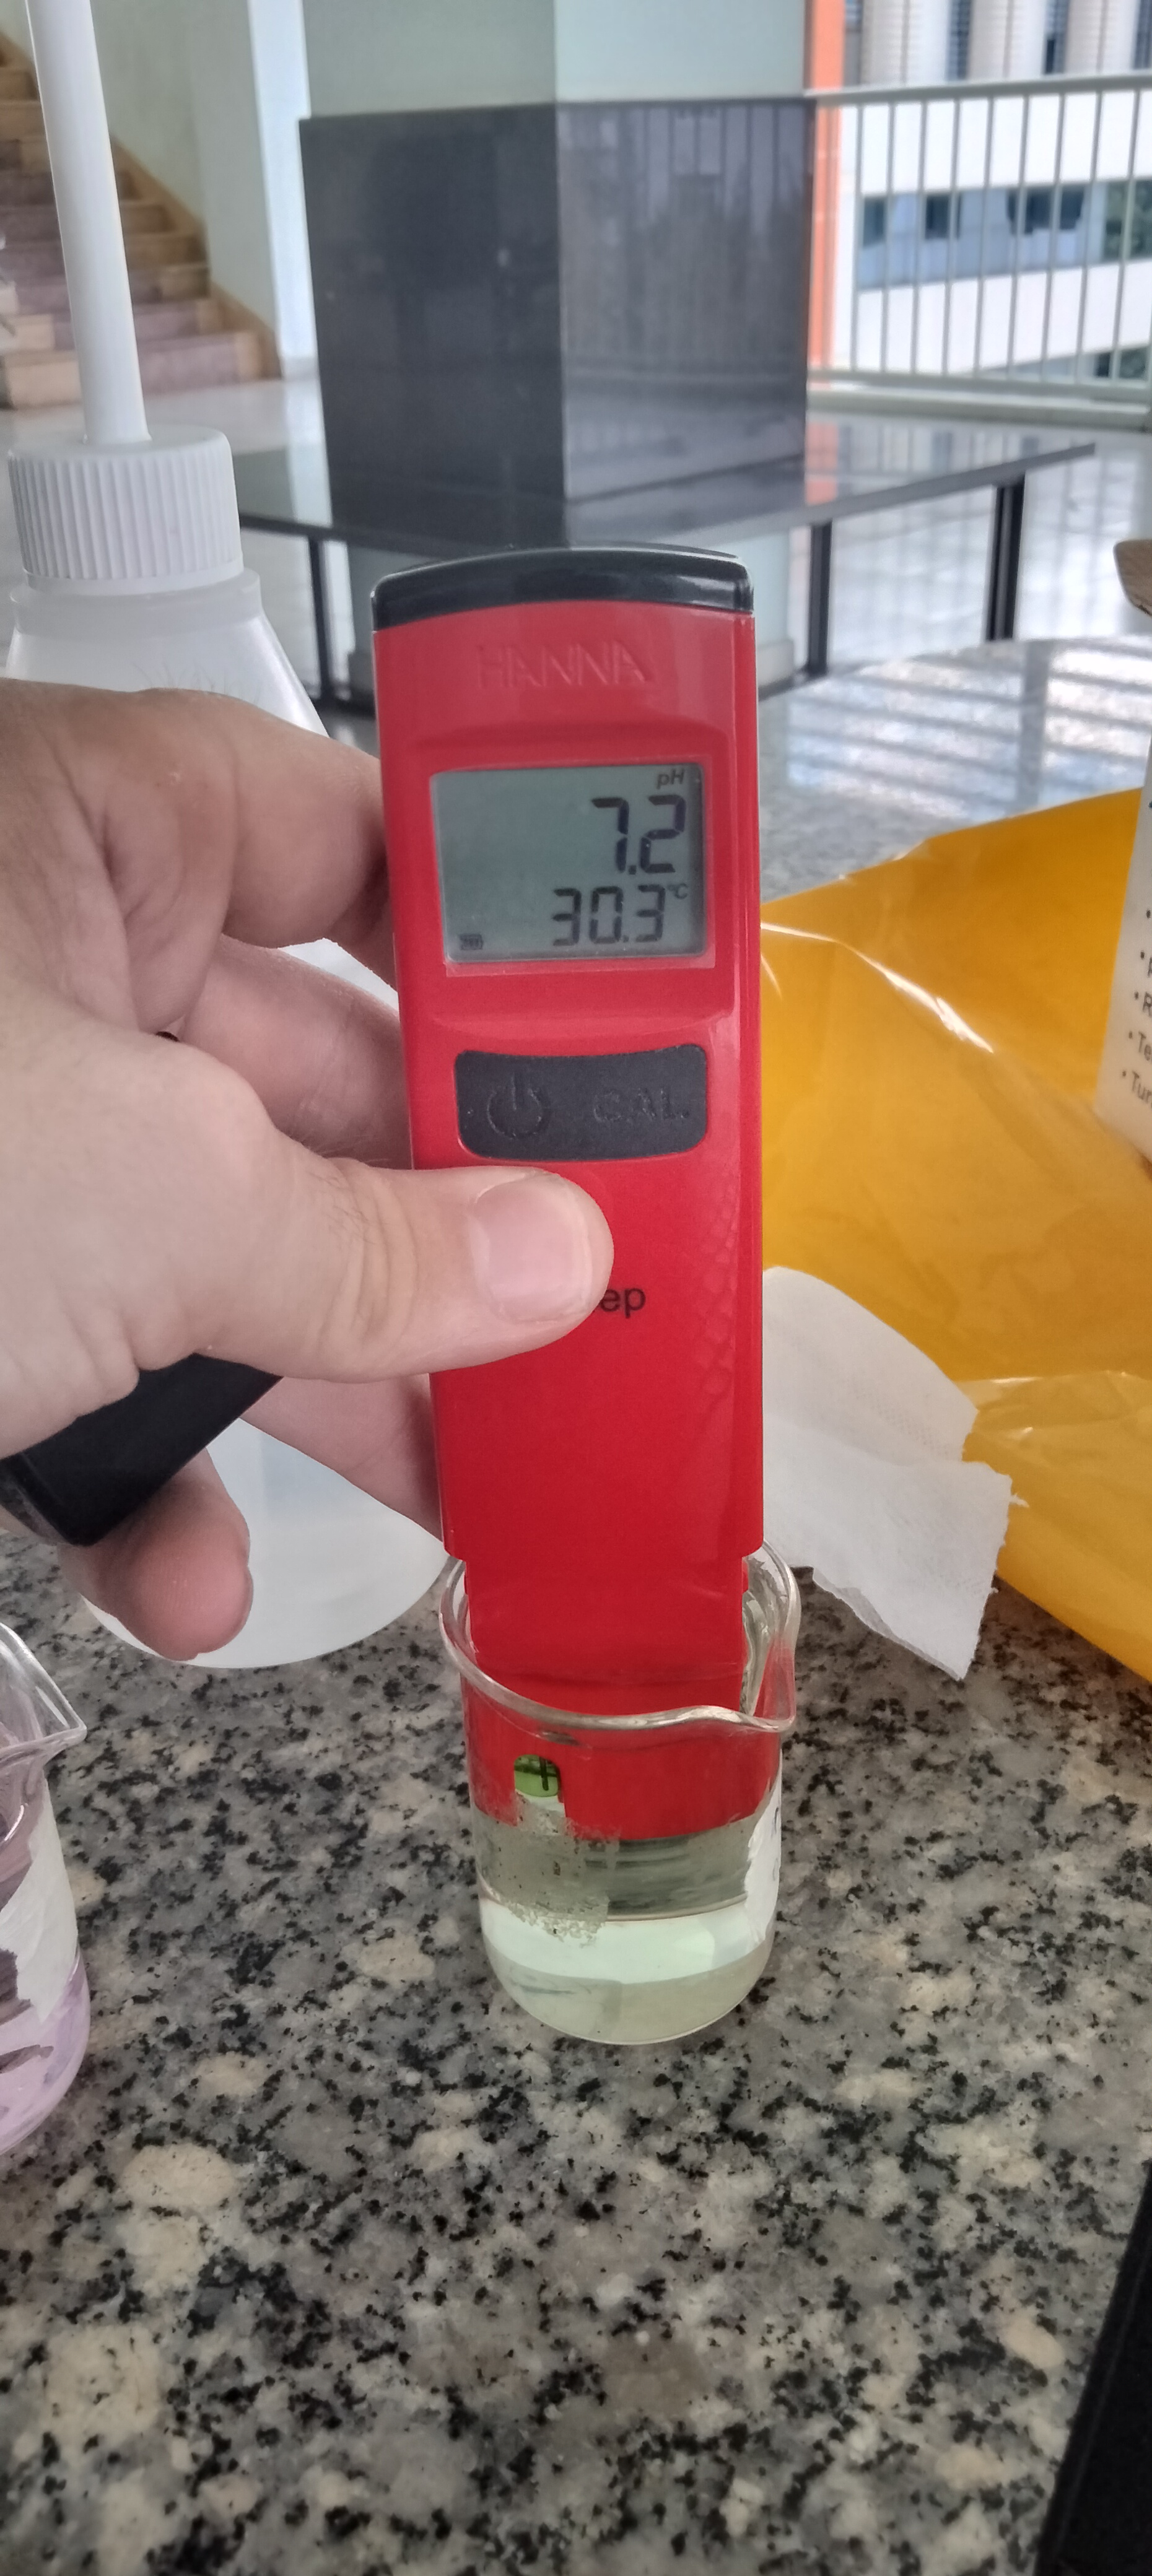
\includegraphics[width=\textwidth]{080_testing/sensors/16_ph7_hanna.jpg}
    \caption{Hanna sensor measuring 7.2}
  \end{minipage}
  \hfill
  \begin{minipage}[b]{0.7\textwidth}
    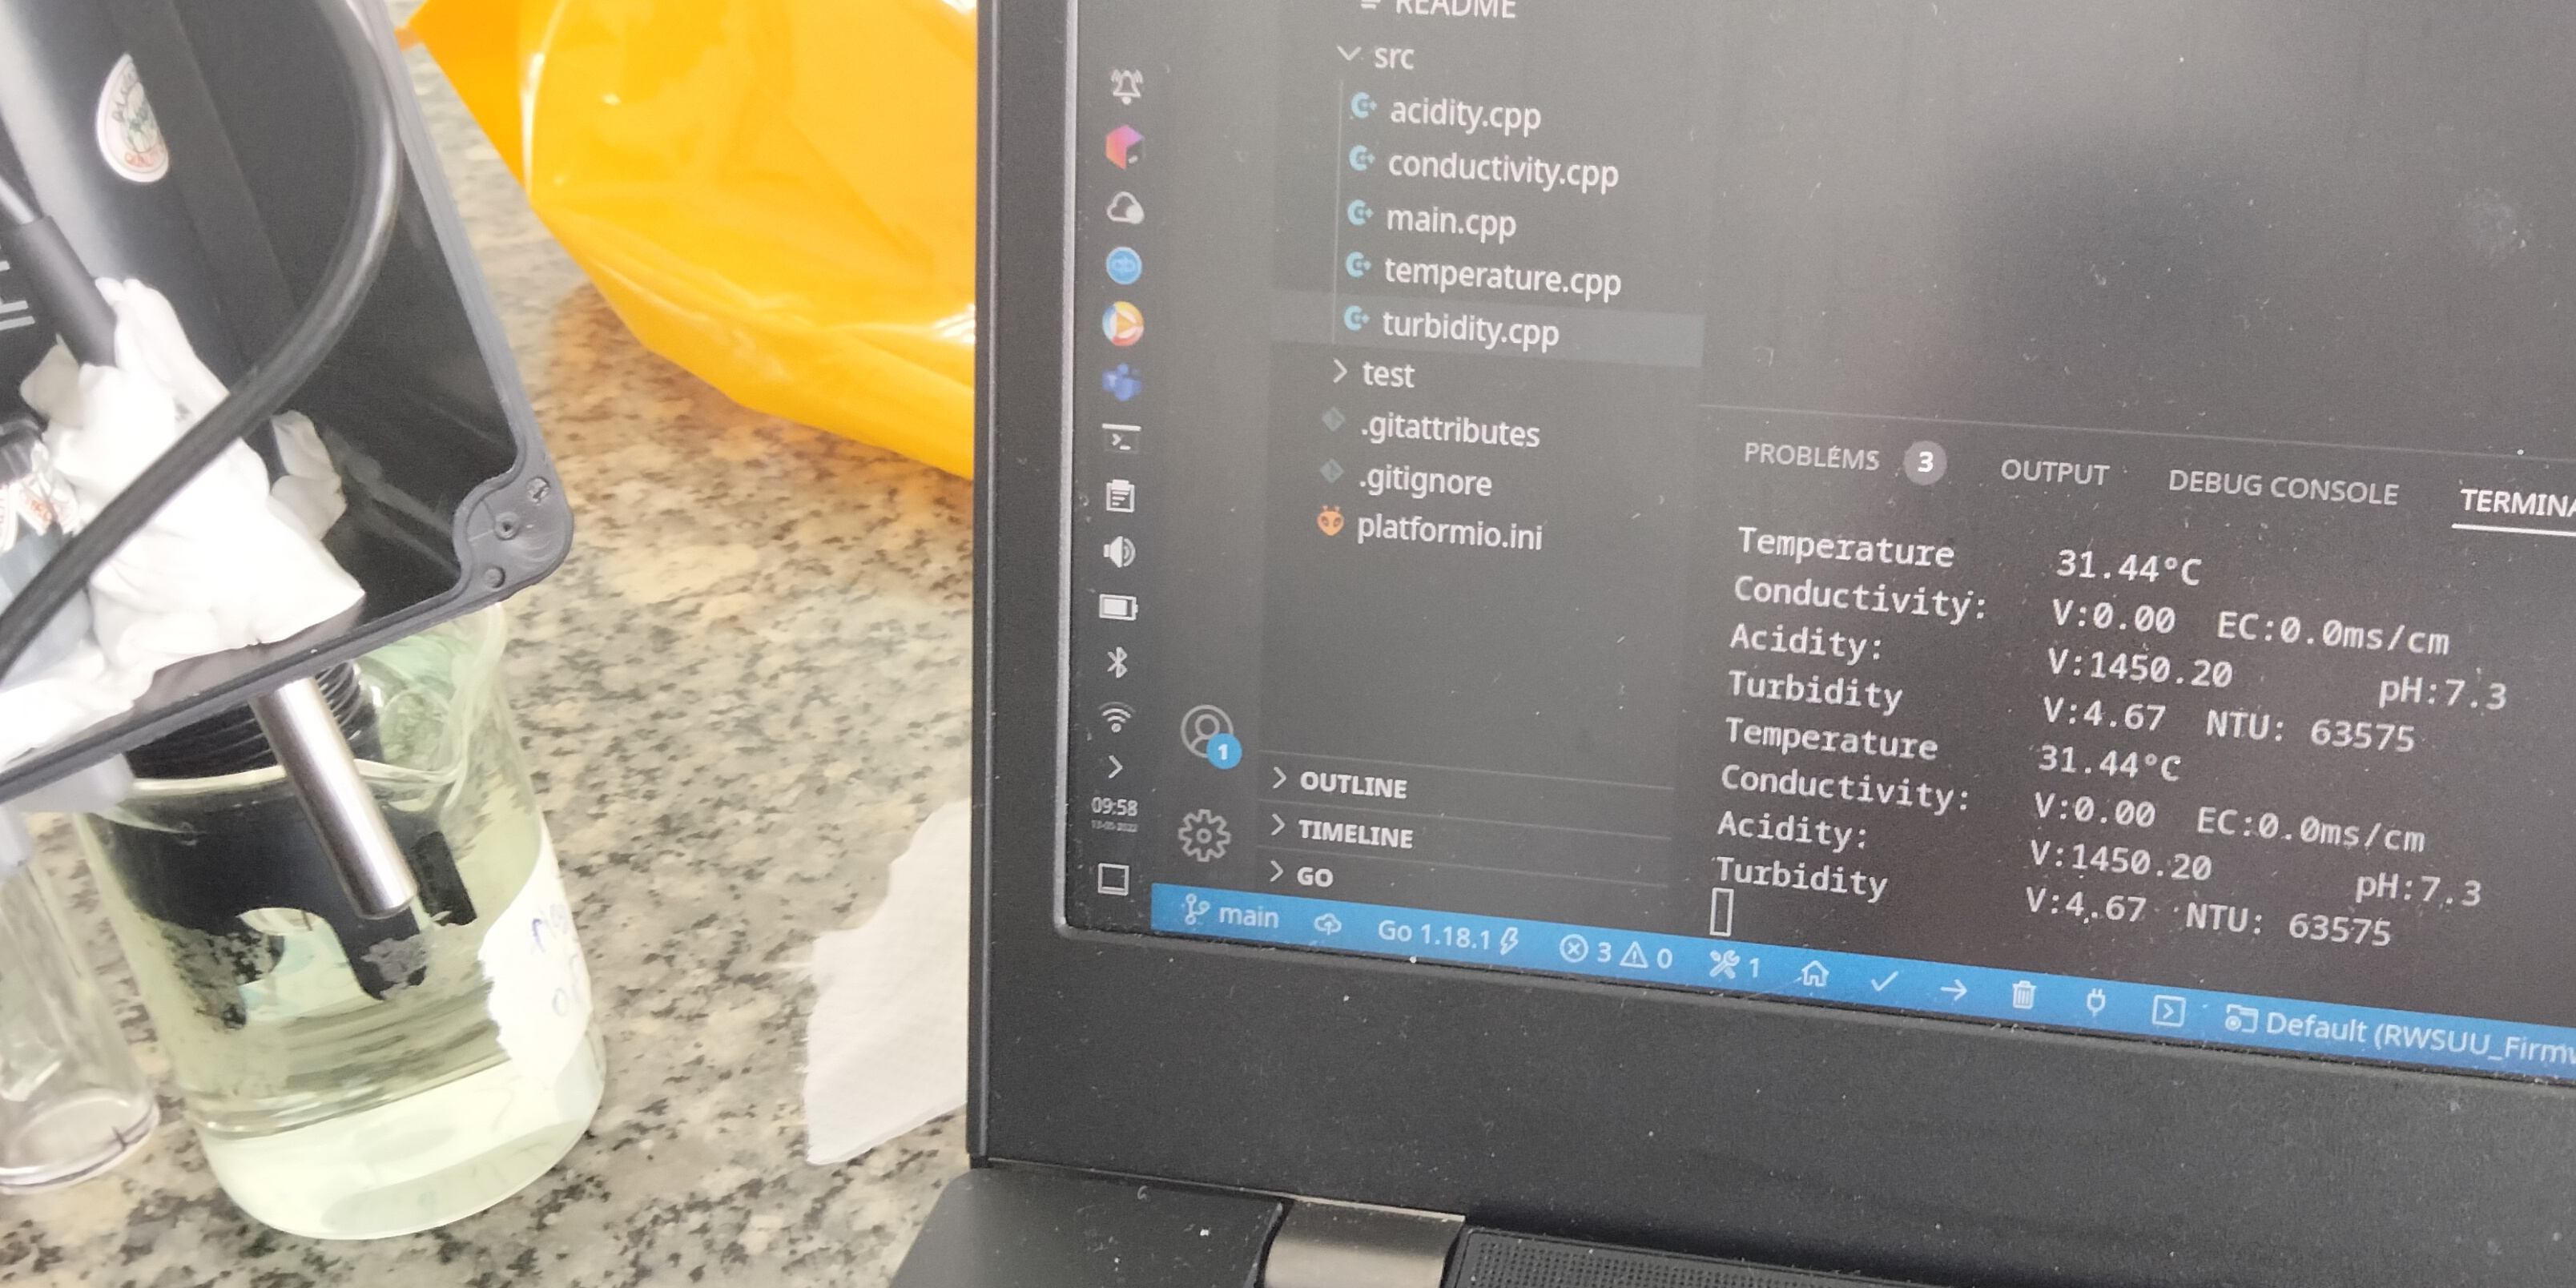
\includegraphics[width=\textwidth]{080_testing/sensors/15_ph7_dfrobot.jpg}
    \caption{DFRobot sensor measuring 7.3}
  \end{minipage}
\end{figure}

\begin{figure}[h!]
\caption{Comparison between Hanna and DFRobot on pH 7.2}
\begin{tikzpicture}
\begin{axis}[
axis lines=middle,
ymin=0,
x label style={at={(current axis.right of origin)},anchor=north, below=10mm},
legend style={at={(0.7,0.7)},anchor=east},
ymin=7, ymax=8,
    xlabel=Samples,
  ylabel=pH,
   enlargelimits = true,
  xticklabels from table={ph4.dat}{Sample},xtick=data]
\addplot[orange,thick,mark=square*] table [y=Hanna,x=X]{ph7.dat};
\addlegendentry{Hanna}
\addplot[green,thick,mark=square*] table [y= DFRobot,x=X]{ph7.dat};
\addlegendentry{DFRobot}]
\end{axis}
\end{tikzpicture}
\end{figure}

As seen in the graph above, the Hanna sensor continously reads 7.2, while the DFRobot sensor continously reads 7.3. The exception is the fourth sample, when the Hanna sensor also read 7.2. This falls into the indicated margin of error.
\newpage
\subsubsection{Conductivity}
As mentioned in the Design Report, the DFRobot DFR0300H \cite{DFR0300H} was chosen for measuring the conductivity. The manufacturer claims the sensor has an accuracy of 5\% \gls{FSR}, meaning with a range of 20\gls{ms}/\gls{cm}, it has an error of 1\gls{ms}/\gls{cm}. Before each sample was taken, the sensor was cleaned with distilled water. A sample is taken a minute after submersion, as the response time of the conductivity sensors are within 1 minute.

\begin{table}[h!]
	\centering
	\adjustimage{height=4cm,valign=c}{080_testing/sensors/23_dfr0300h.jpg}\quad
	\begin{tabular}{| l | l |}
    \hline
    Protocol & Analog\\
    Measurement Accuracy &  5\% FSR\\
    Supply Voltage & 3.3-5V\\
    Support Detection Range & 10~100ms/cm\\
    Software library included & yes \\
    Probe included & yes \\
    Availability & 3-5 Working days \\
    \hline
	\end{tabular}
\end{table}

\paragraph{Known conductivity solutions}
Known conductivity solutions of 12.88\gls{ms}/\gls{cm} and 1.413\gls{ms}/\gls{cm} were used to determine the accuracy of the sensor. These known solutions come from the manufacturer of the sensor and were verified in their lab.

\newpage
\paragraph{First known conductivity solution}
The first solution has a known conductivity of 12.88\gls{ms}/\gls{cm}

\begin{figure}[h]
\centering
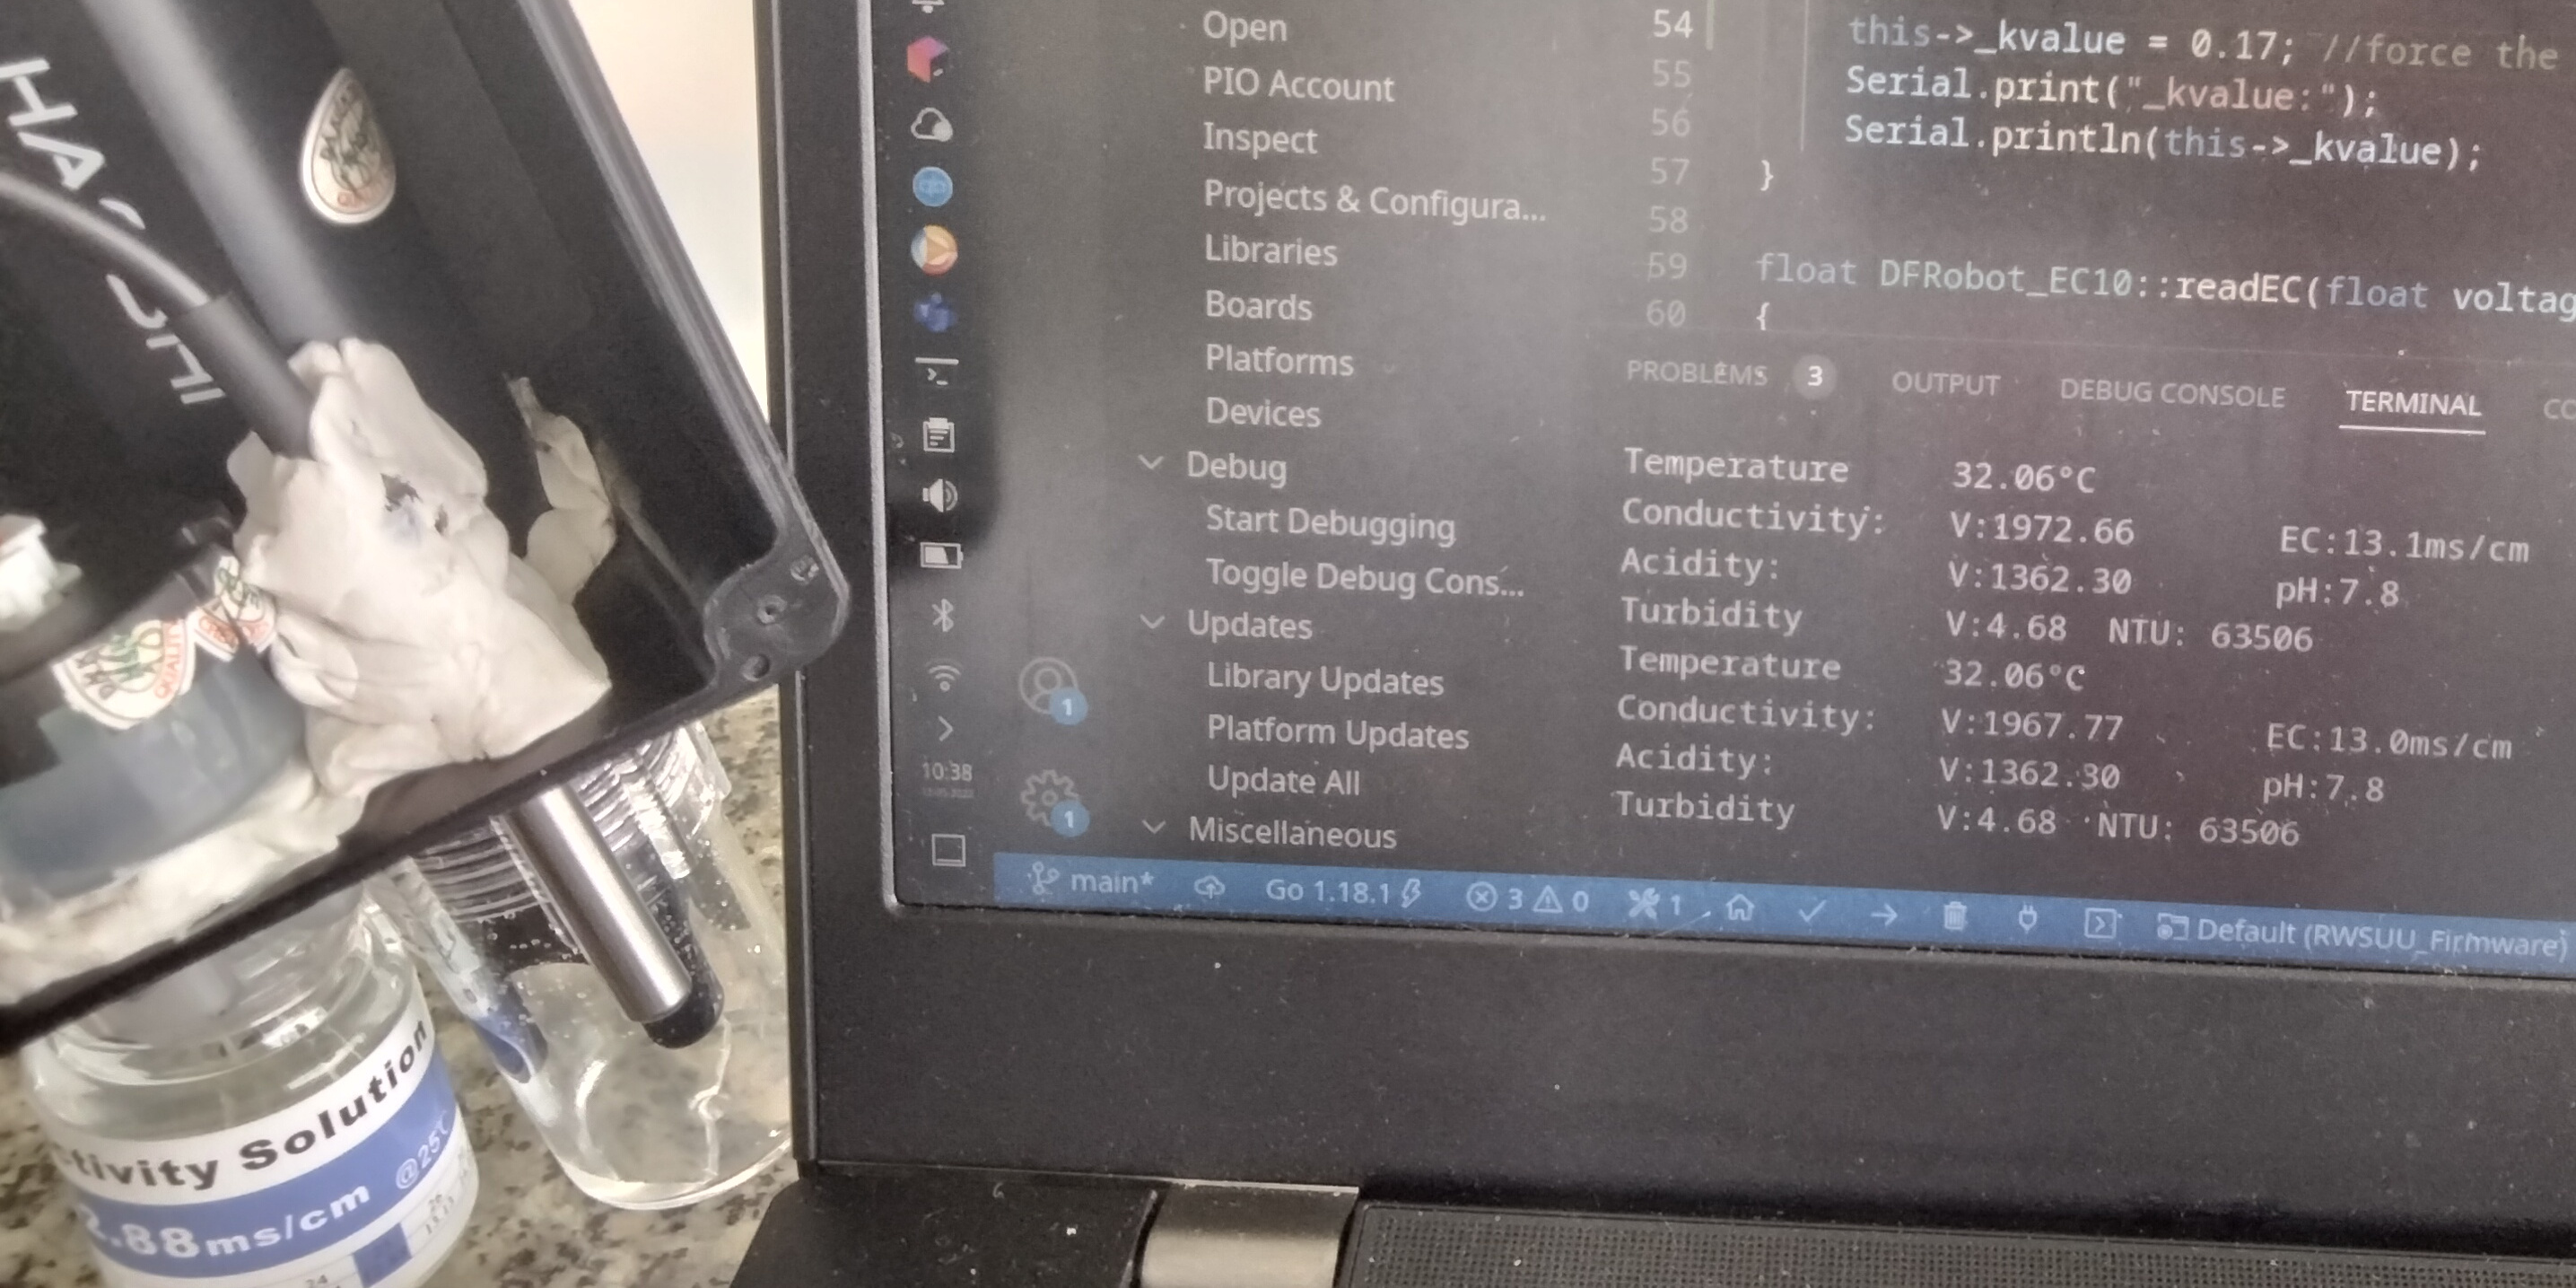
\includegraphics[scale=0.6]{080_testing/sensors/21_ec1288_dfrobot.jpg}
\caption{DFRobot sensor measuring 13.0\gls{ms}/\gls{cm}}
\end{figure}

\begin{figure}[h!]
\caption{DFRobot 13.0\gls{ms}/\gls{cm} samples}
\begin{tikzpicture}
\begin{axis}[
axis lines=middle,
ymin=0,
x label style={at={(current axis.right of origin)},anchor=north, below=10mm},
legend style={at={(0.7,0.7)},anchor=east},
ymin=12, ymax=14,
    xlabel=Samples,
  ylabel=ms/cm,
   enlargelimits = true,
  xticklabels from table={ec1288.dat}{Sample},xtick=data]
\addplot[green,thick,mark=square*] table [y= DFRobot,x=X]{ec1288.dat};
\addlegendentry{DFRobot}]
\addplot[red] table [y= Mean,x=X]{ec1288.dat};
\addlegendentry{mean}]
\end{axis}
\end{tikzpicture}
\end{figure}

As seen in the graph above, all samples fall well within the error range of 1ms/cm. The mean of the samples are 13.06\gls{ms}/\gls{cm}. The sensor performed better than advertised.

\newpage
\paragraph{Second known conductivity solution}
The second solution has a known conductivity of 1.413\gls{ms}/\gls{cm}

\begin{figure}[h]
\centering
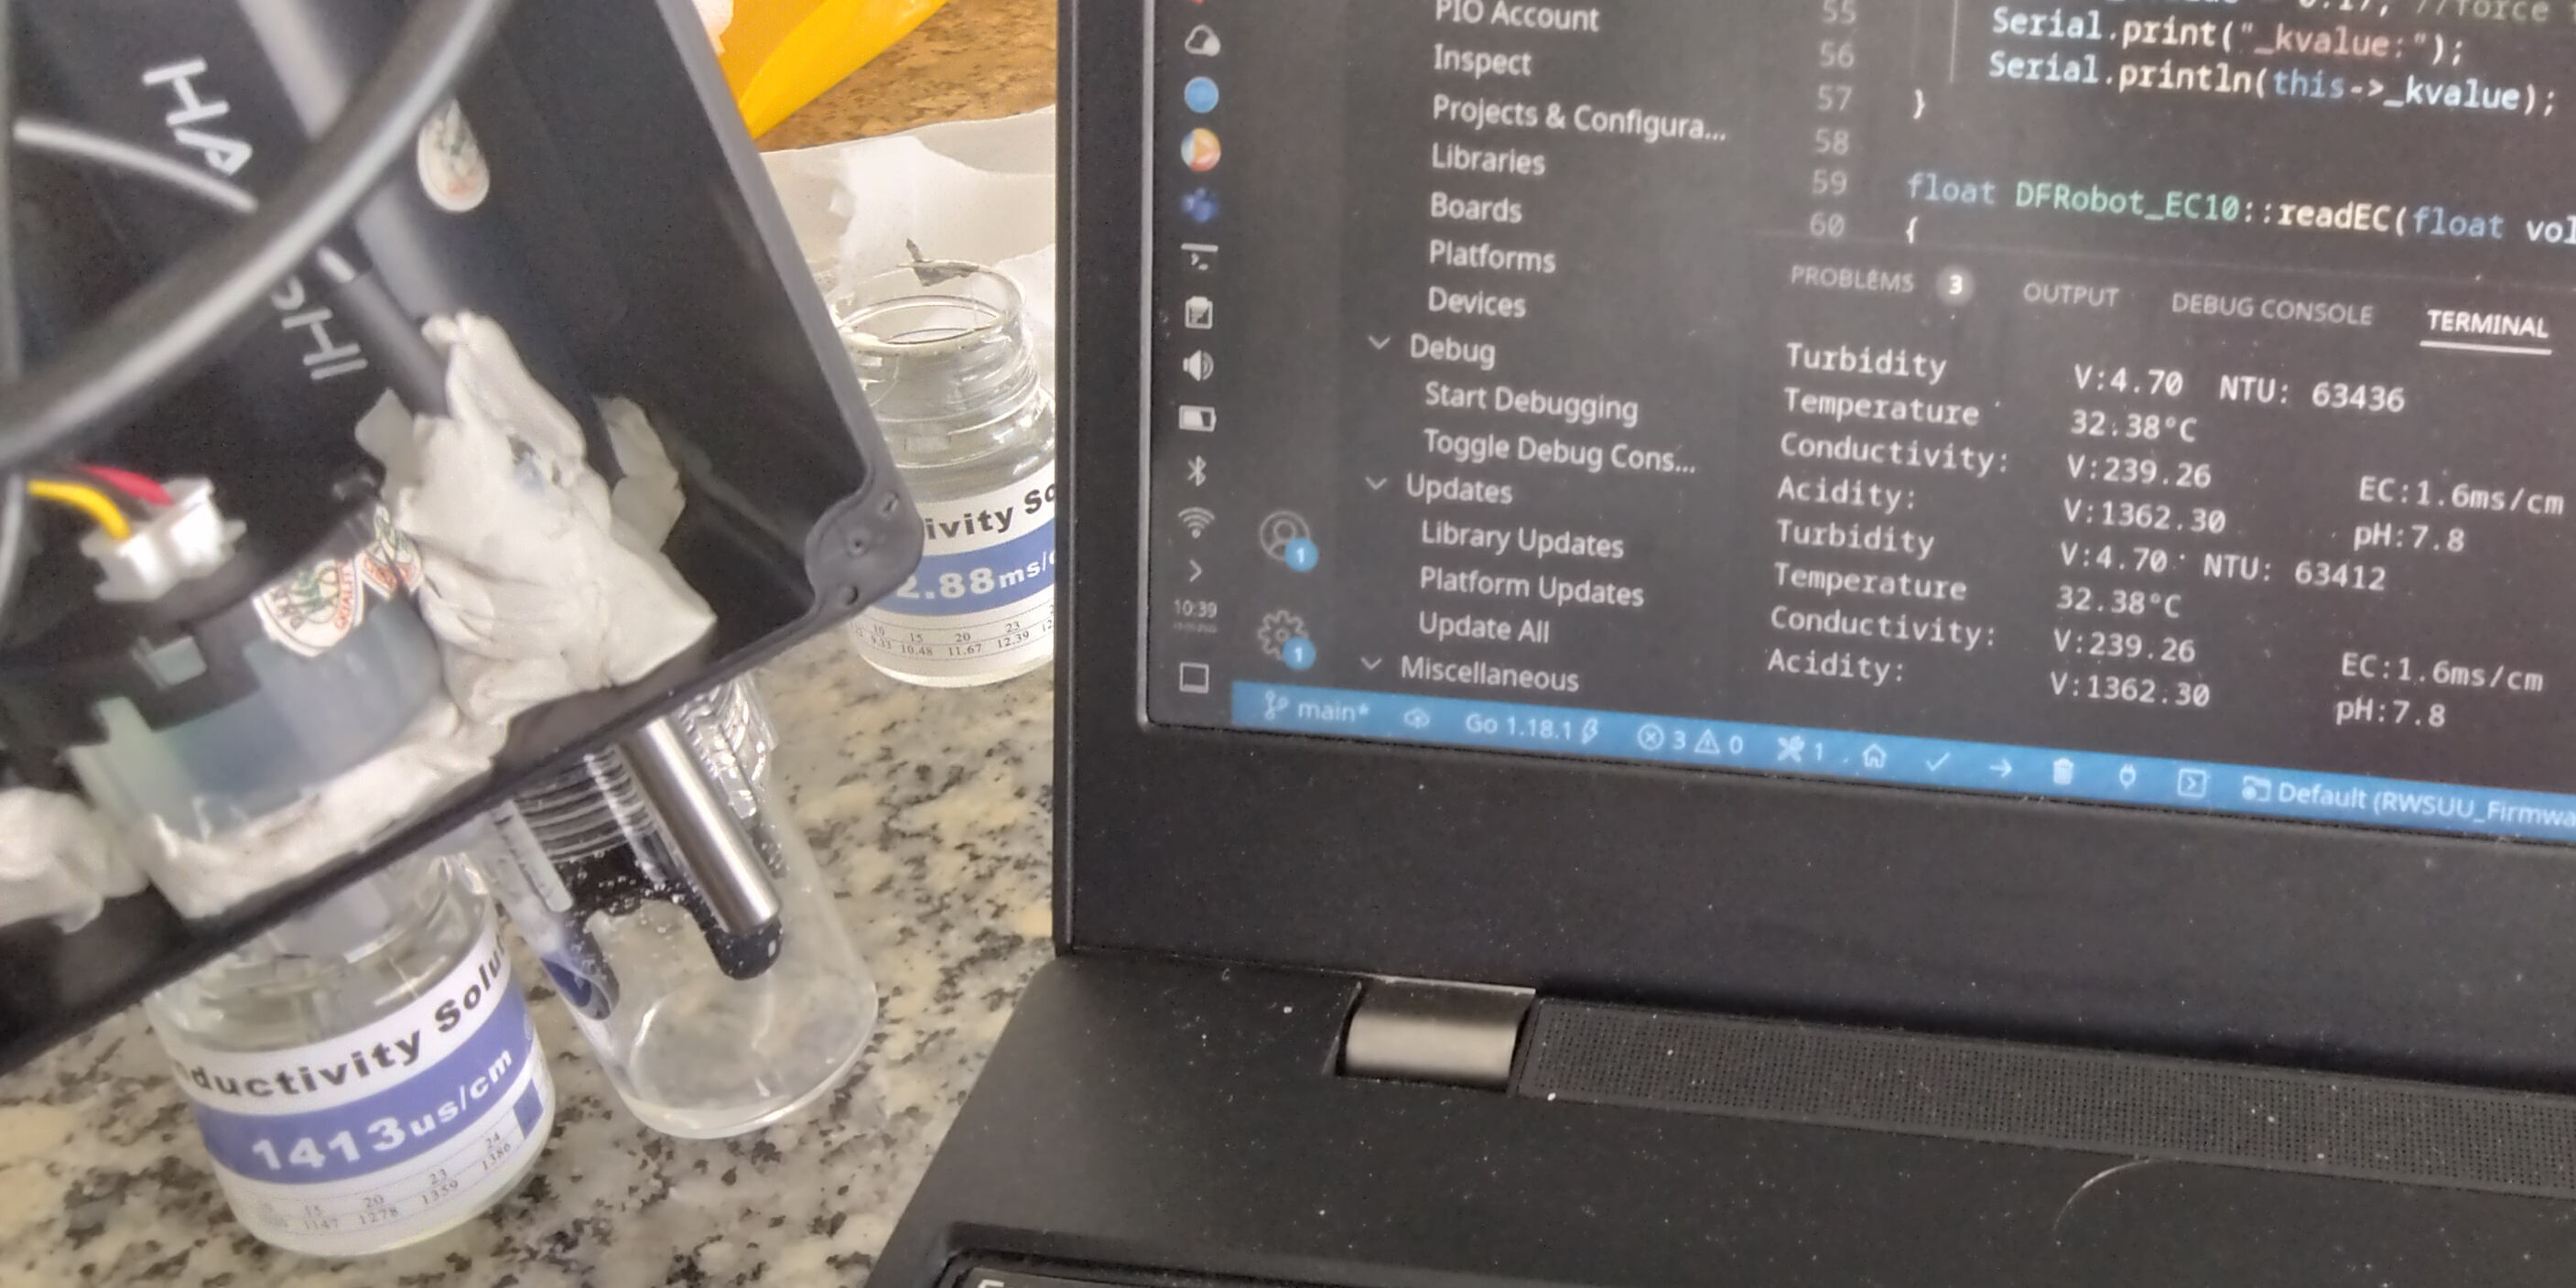
\includegraphics[scale=0.6]{080_testing/sensors/22_ec1413_dfrobot.jpg}
\caption{DFRobot sensor measuring 1.6ms/cm}
\end{figure}

\begin{figure}[h!]
\caption{DFRobot 1.413ms/cm samples}
\begin{tikzpicture}
\begin{axis}[
axis lines=middle,
ymin=0,
x label style={at={(current axis.right of origin)},anchor=north, below=10mm},
legend style={at={(0.7,0.1)},anchor=east},
ymin=1.4, ymax=1.7,
    xlabel=Samples,
  ylabel=ms/cm,
   enlargelimits = true,
  xticklabels from table={ec1433.dat}{Sample},xtick=data]
\addplot[green,thick,mark=square*] table [y= DFRobot,x=X]{ec1433.dat};
\addlegendentry{DFRobot}]
\addplot[red] table [y= Mean,x=X]{ec1433.dat};
\addlegendentry{mean}]
\end{axis}
\end{tikzpicture}
\end{figure}

As seen in the graph above, all samples fall well within the error range of 1\gls{ms}/\gls{cm}. The mean of the samples are 1.56\gls{ms}/\gls{cm}. The sensor performed better than advertised.
\newpage
\subsubsection{Temperature}
As mentioned in the Design Report, the DFRobot DFR0198/DS18B20 \cite{DFR0198} waterproof sensor was chosen to measure the temperature. Temperature readings of the water are both recorded and used to help determining the acidity and conductivity.

\begin{table}[h!]
	\centering
	\adjustimage{height=4cm,valign=c}{080_testing/sensors/31_dfr0198.jpg}\quad
	\begin{tabular}{| l | l |}
    \hline
    Protocol & 1-Wire\\
    Measurement Range & -10-85 ℃ \\
    Measurement Accuracy &  0.5 ℃ \\
    Response time & Within 750ms \\
    Supply Voltage & 3.3V-5V \\
    Software library included & yes \\
    Availability & 3-5 Working Days \\
    \hline
	\end{tabular}
\end{table}

Temperature readings are compared from the Hanna pH sensor and the DFRobot DS18B20 sensor. The Hanna sensor has an accuracy of 1℃ and the DFRobot sensor has an accuracy of 0.5 ℃  The results can be seen in the graph below.

\begin{figure}[h!]
\caption{Comparison between Hanna and DFRobot}
\begin{tikzpicture}
\begin{axis}[
axis lines=middle,
ymin=0,
x label style={at={(current axis.right of origin)},anchor=north, below=10mm},
legend style={at={(1,0.1)},anchor=east},
ymin=29, ymax=33,
    xlabel=Samples,
  ylabel=°C,
   enlargelimits = true,
  xticklabels from table={temp.dat}{Sample},xtick=data]
\addplot[orange,thick,mark=square*] table [y=Hanna,x=X]{temp.dat};
\addlegendentry{Hanna}
\addplot[green,thick,mark=square*] table [y= DFRobot,x=X]{temp.dat};
\addlegendentry{DFRobot}]
\end{axis}
\end{tikzpicture}
\end{figure}

As seen in the graph above, all samples could fall within both error ranges. As the Hanna sensor has a temperature accuracy of only 1℃ it is not possible to determine whether the DFRobot sensor is acting